\documentclass[11pt,a4paper]{report}
\usepackage[textwidth=37em,vmargin=30mm]{geometry}
\usepackage{calc,xunicode,amsmath,amssymb,paralist,enumitem,tabu,booktabs,datetime2,xeCJK,xeCJKfntef,listings}
\usepackage{tocloft,fancyhdr,tcolorbox,xcolor,graphicx,eso-pic,xltxtra,xelatexemoji}

\newcommand{\envyear}[0]{2025}
\newcommand{\envdatestr}[0]{2025-10-13}
\newcommand{\envfinaldir}[0]{webdb/2025/20251013/final}

\usepackage[hidelinks]{hyperref}
\hypersetup{
    colorlinks=false,
    pdfpagemode=FullScreen,
    pdftitle={Web Digest - \envdatestr}
}

\setlength{\cftbeforechapskip}{10pt}
\renewcommand{\cftchapfont}{\rmfamily\bfseries\large\raggedright}
\setlength{\cftbeforesecskip}{2pt}
\renewcommand{\cftsecfont}{\sffamily\small\raggedright}

\setdefaultleftmargin{2em}{2em}{1em}{1em}{1em}{1em}

\usepackage{xeCJK,xeCJKfntef}
\xeCJKsetup{PunctStyle=plain,RubberPunctSkip=false,CJKglue=\strut\hskip 0pt plus 0.1em minus 0.05em,CJKecglue=\strut\hskip 0.22em plus 0.2em}
\XeTeXlinebreaklocale "zh"
\XeTeXlinebreakskip = 0pt


\setmainfont{Brygada 1918}
\setromanfont{Brygada 1918}
\setsansfont{IBM Plex Sans}
\setmonofont{JetBrains Mono NL}
\setCJKmainfont{Noto Serif CJK SC}
\setCJKromanfont{Noto Serif CJK SC}
\setCJKsansfont{Noto Sans CJK SC}
\setCJKmonofont{Noto Sans CJK SC}

\setlength{\parindent}{0pt}
\setlength{\parskip}{8pt}
\linespread{1.15}

\lstset{
	basicstyle=\ttfamily\footnotesize,
	numbersep=5pt,
	backgroundcolor=\color{black!5},
	showspaces=false,
	showstringspaces=false,
	showtabs=false,
	tabsize=2,
	captionpos=b,
	breaklines=true,
	breakatwhitespace=true,
	breakautoindent=true,
	linewidth=\textwidth
}






\newcommand{\coverpic}[2]{
    % argv: itemurl, authorname
    Cover photo by #2~~(\href{#1}{#1})
}
\newcommand{\makeheader}[0]{
    \begin{titlepage}
        % \newgeometry{hmargin=15mm,tmargin=21mm,bmargin=12mm}
        \begin{center}
            
            \rmfamily\scshape
            \fontspec{BaskervilleF}
            \fontspec{Old Standard}
            \fontsize{59pt}{70pt}\selectfont
            WEB\hfill DIGEST
            
            \vfill
            % \vskip 30pt
            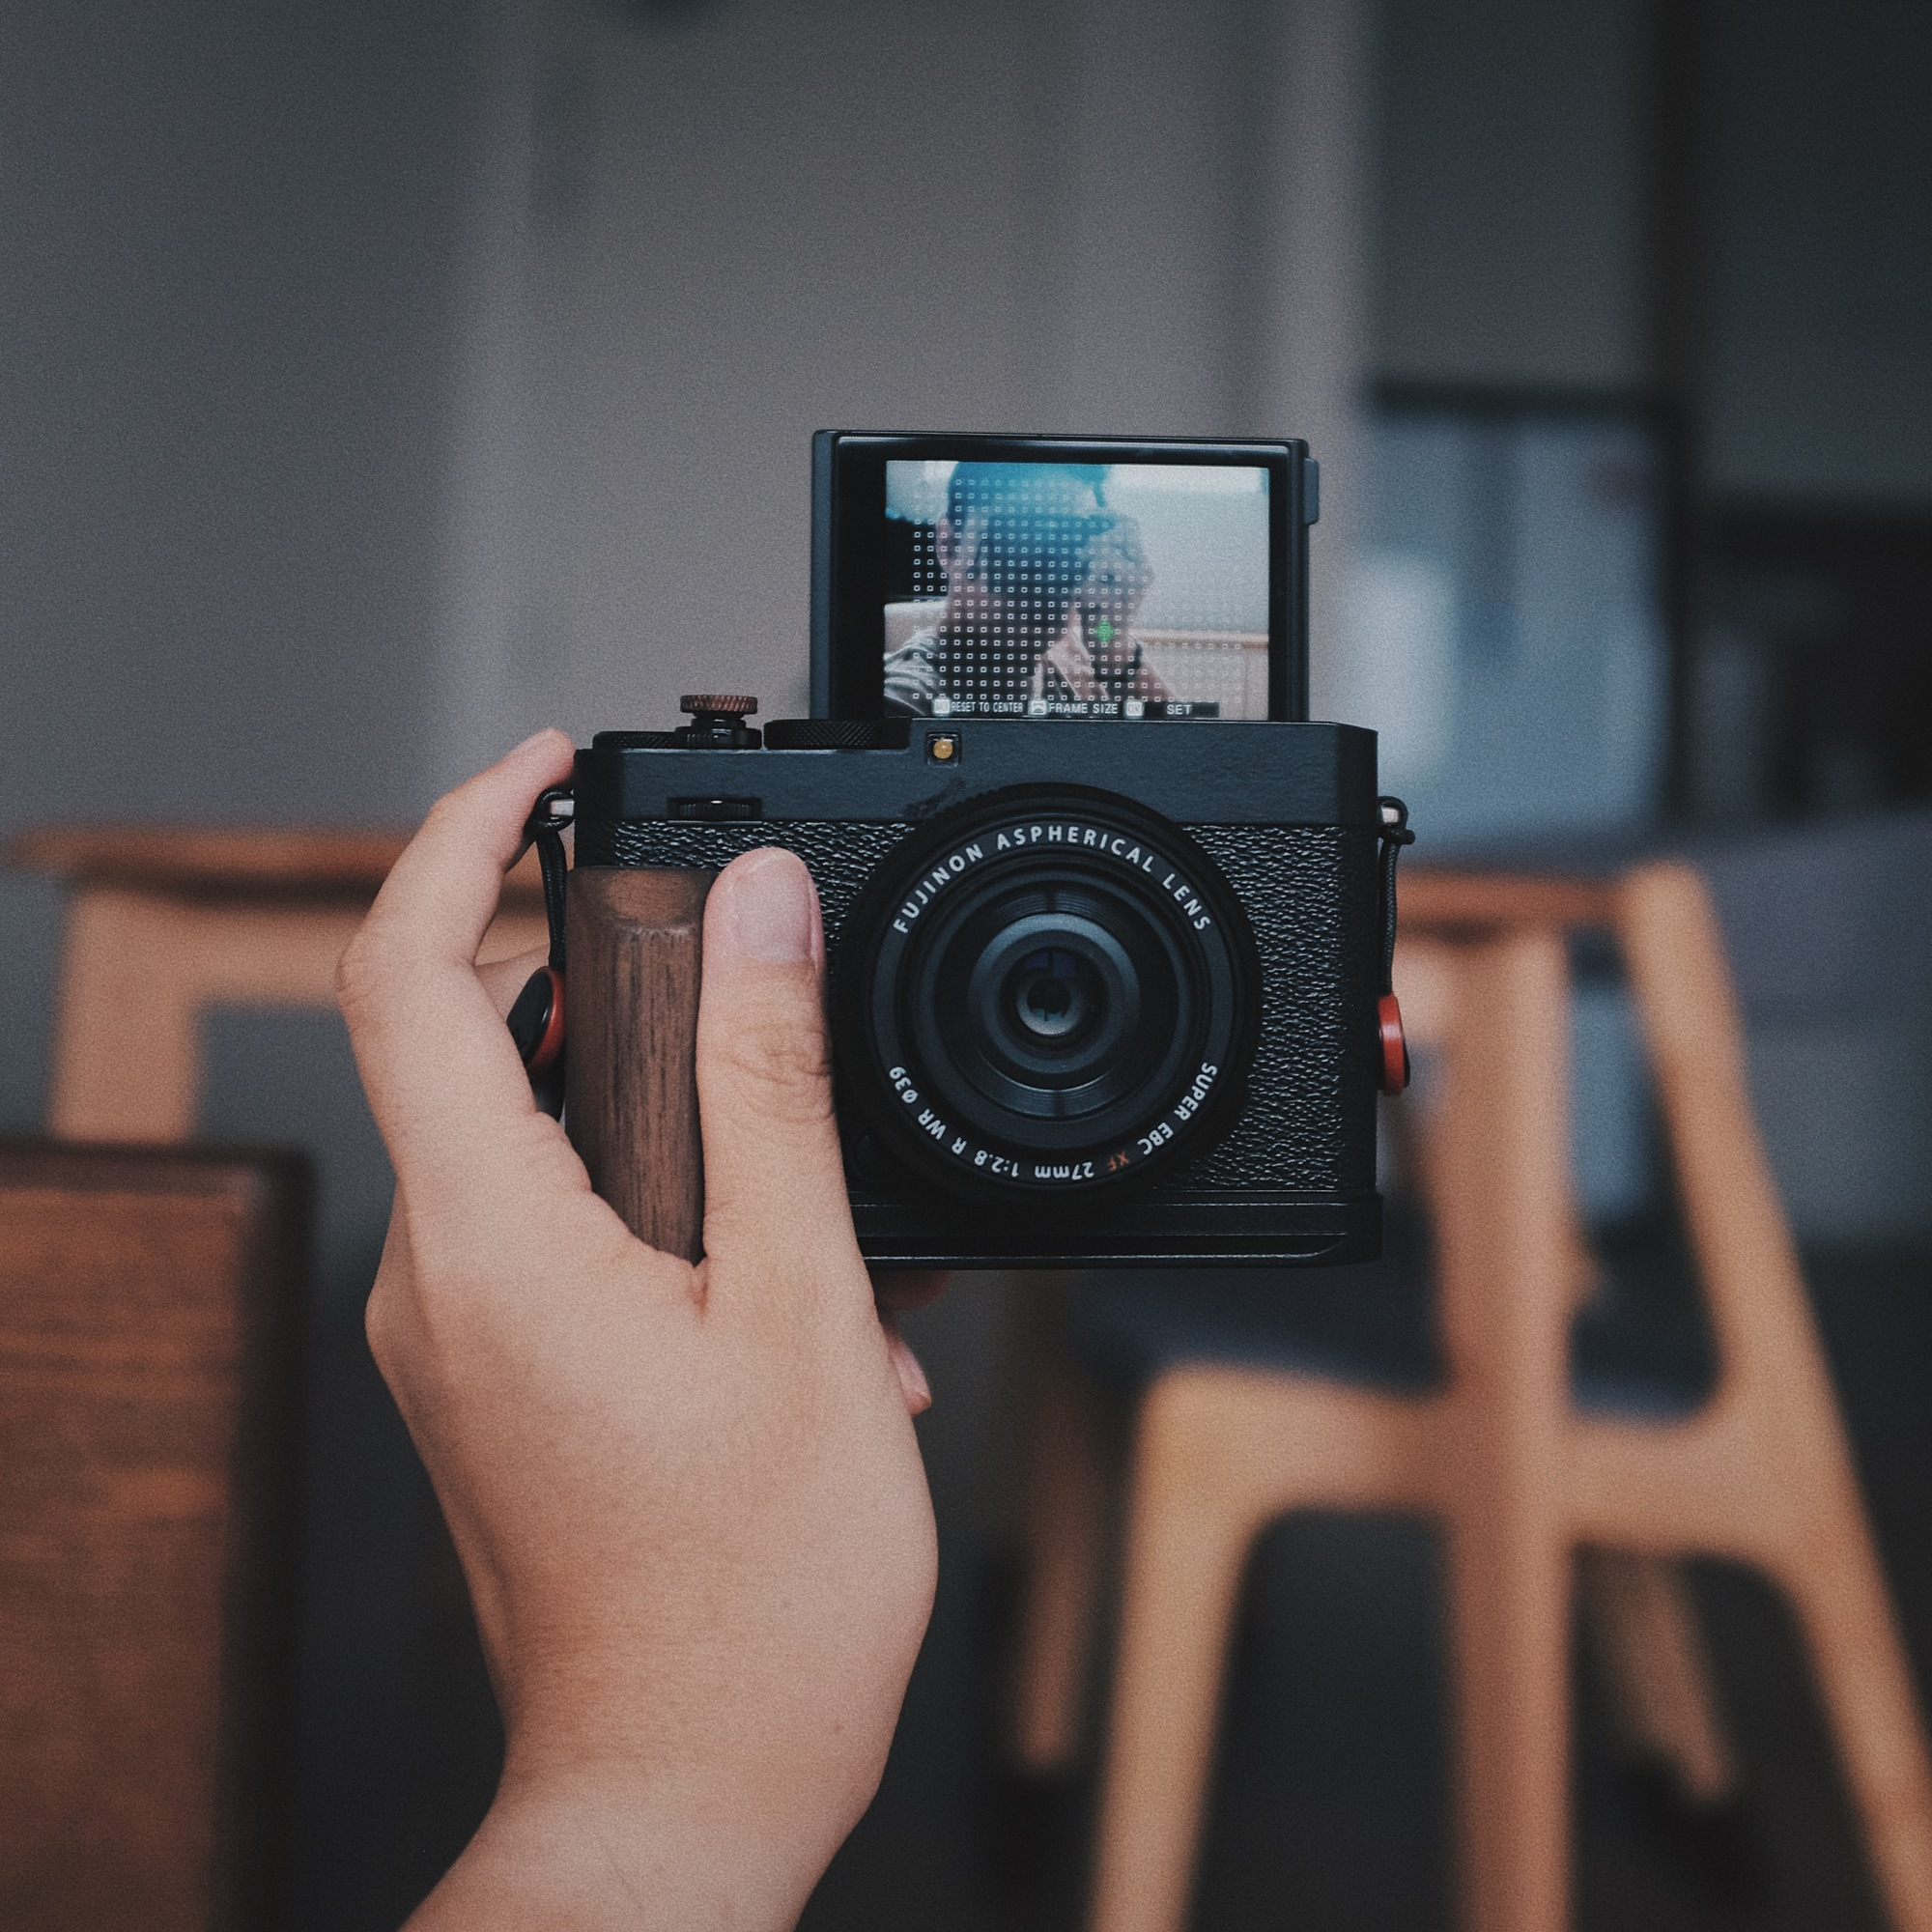
\includegraphics[width=\linewidth]{\envfinaldir/coverpic-prod.jpg}\par
            % \vskip 30pt
            \vfill

            \normalsize\rmfamily\scshape
            \copyright{} The Web Digest Project \hfill\large \envdatestr
        \end{center}
    \end{titlepage}
    % \restoregeometry
}
\newcommand{\simplehref}[1]{%
    \textcolor{blue!80!green}{\href{#1}{#1}}%
}
\renewcommand{\contentsname}{\center\Huge\sffamily\bfseries Contents\par\vskip 20pt}
\newcounter{ipartcounter}
\setcounter{ipartcounter}{0}
\newcommand{\ipart}[1]{
    % \vskip 20pt
    \clearpage
    \stepcounter{ipartcounter}
    \phantomsection
    \addcontentsline{toc}{chapter}{#1}
    % \begin{center}
    %     \Huge
    %     \sffamily\bfseries
    %     #1
    % \end{center}
    % \vskip 20pt plus 7pt
}
\newcounter{ichaptercounter}
\setcounter{ichaptercounter}{0}
\newcommand{\ichapter}[1]{
    % \vskip 20pt
    \clearpage
    \stepcounter{ichaptercounter}
    \phantomsection
    \addcontentsline{toc}{section}{\numberline{\arabic{ichaptercounter}}#1}
    \begin{center}
        \Huge
        \sffamily\bfseries
        #1
    \end{center}
    \vskip 20pt plus 7pt
}
\newcommand{\entrytitlefont}[1]{\subsection*{\raggedright\Large\sffamily\bfseries#1}}
\newcommand{\entryitemGeneric}[2]{
    % argv: title, url
    \parbox{\linewidth}{
        \entrytitlefont{#1}\par\vskip 5pt
        \footnotesize\ttfamily\mdseries
        \simplehref{#2}
    }\vskip 11pt plus 11pt minus 1pt
}
\newcommand{\entryitemGithub}[3]{
    % argv: title, url, desc
    \parbox{\linewidth}{
        \entrytitlefont{#1}\par\vskip 5pt
        \footnotesize\ttfamily\mdseries
        \simplehref{#2}\par\vskip 5pt
        \small\rmfamily\mdseries#3
    }\vskip 11pt plus 11pt minus 1pt
}
\newcommand{\entryitemAp}[3]{
    % argv: title, url, desc
    \parbox{\linewidth}{
        \entrytitlefont{#1}\par\vskip 5pt
        \footnotesize\ttfamily\mdseries
        \simplehref{#2}\par\vskip 5pt
        \small\rmfamily\mdseries#3
    }\vskip 11pt plus 11pt minus 1pt
}
\newcommand{\entryitemHackernews}[3]{
    % argv: title, hnurl, rawurl
    % \parbox{\linewidth}{
    %     \entrytitlefont{#1}\par\vskip 5pt
    %     \footnotesize\ttfamily\mdseries
    %     \simplehref{#3}\par
    %     \textcolor{black!50}{\href{#2}{#2}}
    % }\vskip 11pt plus 11pt minus 1pt
    \begin{minipage}{\linewidth}
            \entrytitlefont{#1}\par\vskip 5pt
            \footnotesize\ttfamily\mdseries
            \simplehref{#3}\par
            \textcolor{black!50}{\href{#2}{#2}}
    \end{minipage}\par\vskip 11pt plus 11pt minus 1pt
}







\begin{document}

\makeheader

\tableofcontents\clearpage




\ipart{Developers}
\ichapter{Hacker News}
\entryitemTwoLinks{After the AI boom: what might we be left with?}{https://news.ycombinator.com/item?id=45561164}{https://blog.robbowley.net/2025/10/12/after-the-ai-boom-what-might-we-be-left-with/}

\entryitemTwoLinks{Wireguard FPGA}{https://news.ycombinator.com/item?id=45559857}{https://github.com/chili-chips-ba/wireguard-fpga}

\entryitemTwoLinks{'Death to Spotify': the DIY movement to get artists and fans to quit the app}{https://news.ycombinator.com/item?id=45559852}{https://www.theguardian.com/technology/2025/oct/12/spotify-boycott-artists}

\entryitemTwoLinks{GitHub Copilot: Remote Code Execution via Prompt Injection (CVE-2025-53773)}{https://news.ycombinator.com/item?id=45559603}{https://embracethered.com/blog/posts/2025/github-copilot-remote-code-execution-via-prompt-injection/}

\entryitemTwoLinks{In 1776, Thomas Paine made the best case for fighting kings −and being skeptical}{https://news.ycombinator.com/item?id=45559567}{https://theconversation.com/in-1776-thomas-paine-made-the-best-case-for-fighting-kings-and-for-being-skeptical-266448}

\entryitemTwoLinks{Addictive-like behavioural traits in pet dogs with extreme motivation for toys}{https://news.ycombinator.com/item?id=45559305}{https://www.nature.com/articles/s41598-025-18636-0}

\entryitemTwoLinks{How I'm using Helix editor}{https://news.ycombinator.com/item?id=45559076}{https://rushter.com/blog/helix-editor/}

\entryitemTwoLinks{No I don't want to turn on Windows Backup with One Drive}{https://news.ycombinator.com/item?id=45559023}{https://idiallo.com/byte-size/say-no-to-onedrive-backup}

\entryitemTwoLinks{Schleswig-Holstein completes migration to open source email}{https://news.ycombinator.com/item?id=45558635}{https://news.itsfoss.com/schleswig-holstein-email-system-migration/}

\entryitemTwoLinks{Jeep pushed software update that bricked all 2024 Wrangler 4xe models}{https://news.ycombinator.com/item?id=45558318}{https://twitter.com/StephenGutowski/status/1977055831720862101}

\entryitemTwoLinks{Quantification of fibrinaloid clots in plasma from pediatric Long COVID patients}{https://news.ycombinator.com/item?id=45557267}{https://www.researchsquare.com/article/rs-7483367/v1}

\entryitemTwoLinks{Why Wikipedia cannot claim the Earth is not flat}{https://news.ycombinator.com/item?id=45557013}{https://en.wikipedia.org/wiki/Wikipedia:Why\_Wikipedia\_cannot\_claim\_the\_Earth\_is\_not\_flat}

\entryitemTwoLinks{Macro Splats 2025}{https://news.ycombinator.com/item?id=45556952}{https://danybittel.ch/macro.html}

\entryitemTwoLinks{Nostr and ATProto (2024)}{https://news.ycombinator.com/item?id=45556763}{https://shreyanjain.net/2024/07/05/nostr-and-atproto.html}

\entryitemTwoLinks{Why it took 4 years to get a lock files specification}{https://news.ycombinator.com/item?id=45556741}{https://snarky.ca/why-it-took-4-years-to-get-a-lock-files-specification/}

\entryitemTwoLinks{AdapTive-LeArning Speculator System (ATLAS): Faster LLM inference}{https://news.ycombinator.com/item?id=45556474}{https://www.together.ai/blog/adaptive-learning-speculator-system-atlas}

\entryitemTwoLinks{The App Store was always authoritarian}{https://news.ycombinator.com/item?id=45556032}{https://infrequently.org/2025/10/the-app-store-was-always-authoritarian/}

\entryitemTwoLinks{Spyware maker NSO Group confirms acquisition by US investors}{https://news.ycombinator.com/item?id=45555570}{https://techcrunch.com/2025/10/10/spyware-maker-nso-group-confirms-acquisition-by-us-investors/}

\entryitemTwoLinks{Show HN: I made an esoteric programming language that's read like a spellbook}{https://news.ycombinator.com/item?id=45555523}{https://github.com/sirbread/spellscript}

\entryitemTwoLinks{Pipelining in psql (PostgreSQL 18)}{https://news.ycombinator.com/item?id=45555308}{https://postgresql.verite.pro/blog/2025/10/01/psql-pipeline.html}\ichapter{Phoronix}
\entryitemGeneric{\hskip 0pt{}Linux 6.18-rc1 Released With New Tyr \& Rocket Drivers, Haptic Touchpads \& DM-PCACHE}{https://www.phoronix.com/news/Linux-6.18-rc1-Released}

\entryitemGeneric{\hskip 0pt{}CLUDA Posted For Mesa: Gallium3D API Implemented Atop NVIDIA CUDA Driver API}{https://www.phoronix.com/news/Mesa-CLUDA-MR-CUDA-Gallium}

\entryitemGeneric{\hskip 0pt{}Intel Posts Patches For New VFIO Xe PCI Linux Driver}{https://www.phoronix.com/news/Intel-VFIO-Xe-PCI-Driver-Linux}

\entryitemGeneric{\hskip 0pt{}Linux Patches Posted For Microsoft's ACPI Fan Extensions}{https://www.phoronix.com/news/Linux-Microsoft-ACPI-Fan}

\entryitemGeneric{\hskip 0pt{}Git Developers Talk About Potentially Releasing Git 3.0 By The End Of Next Year}{https://www.phoronix.com/news/Git-3.0-Release-Talk-2026}

\entryitemGeneric{\hskip 0pt{}FreeBSD 15.0 Beta 1 Brings OpenZFS Upgrade, Performance Fix For TCP LRO}{https://www.phoronix.com/news/FreeBSD-15.0-Beta-1}

\entryitemGeneric{\hskip 0pt{}Imagination PowerVR Mesa Vulkan Driver Enables Unofficial Support For More GPUs}{https://www.phoronix.com/news/PowerVR-Mesa-More-GPUs}

\entryitemGeneric{\hskip 0pt{}Linux 6.18 Lands Retpoline Optimization To Help With Intel E Cores}{https://www.phoronix.com/news/Linux-6.18-Retpoline-Opt}

\entryitemGeneric{\hskip 0pt{}Solus Linux Preparing To Remove Python 2, Big systemd Upgrade \& Finish /usr Merge}{https://www.phoronix.com/news/Solus-Linux-EOY-2025-Epoch}


\ipart{Developers~~~~(zh-Hans)}
\ichapter{Solidot}
\entryitemGeneric{\hskip 0pt{}小鼠实验显示新癌症疫苗疗效显著}{https://www.solidot.org/story?sid=82521}

\entryitemGeneric{\hskip 0pt{}海关严查英伟达 AI 芯片}{https://www.solidot.org/story?sid=82520}

\entryitemGeneric{\hskip 0pt{}波兰称针对其关键基础设施的网络攻击在增加}{https://www.solidot.org/story?sid=82519}

\entryitemGeneric{\hskip 0pt{}我国成年人日均锌摄入量呈下降趋势}{https://www.solidot.org/story?sid=82518}

\entryitemGeneric{\hskip 0pt{}逾半数富有企业家考虑移民}{https://www.solidot.org/story?sid=82517}

\entryitemGeneric{\hskip 0pt{}ESA 报告称玩家的平均年龄 41 岁}{https://www.solidot.org/story?sid=82516}

\entryitemGeneric{\hskip 0pt{}研究发现让大模型中毒非常容易}{https://www.solidot.org/story?sid=82515}

\entryitemGeneric{\hskip 0pt{}微软开发者披露臭名昭著的 FCKGW 密钥来历}{https://www.solidot.org/story?sid=82514}

\entryitemGeneric{\hskip 0pt{}英特尔重新思考其开源战略}{https://www.solidot.org/story?sid=82513}

\entryitemGeneric{\hskip 0pt{}日全食期间鸟类行为发生改变}{https://www.solidot.org/story?sid=82512}

\entryitemGeneric{\hskip 0pt{}天文学家使用引力透镜发现最小的暗天体}{https://www.solidot.org/story?sid=82511}

\entryitemGeneric{\hskip 0pt{}裸鼹鼠长寿的秘密可能在于其 DNA 修复机制}{https://www.solidot.org/story?sid=82510}

\entryitemGeneric{\hskip 0pt{}GitHub 正将其基础设施迁移到 Azure}{https://www.solidot.org/story?sid=82509}

\entryitemGeneric{\hskip 0pt{}英国央行对 AI 泡沫破裂发出警告}{https://www.solidot.org/story?sid=82508}

\entryitemGeneric{\hskip 0pt{}空客 A320 交付量超过波音 737}{https://www.solidot.org/story?sid=82507}

\entryitemGeneric{\hskip 0pt{}日本公司本月将把酿酒设备送到国际空间站}{https://www.solidot.org/story?sid=82506}

\entryitemGeneric{\hskip 0pt{}DC 漫画称不会支持 AI 创作}{https://www.solidot.org/story?sid=82505}\ichapter{V2EX}
\entryitemGeneric{\hskip 0pt{}[问与答] 拜托🙏🏻,懂酒的朋友进来看下,为什么京东这两个价格差别这么大?}{https://www.v2ex.com/t/1164715}

\entryitemGeneric{\hskip 0pt{}[程序员] cursor 是不是涨价了}{https://www.v2ex.com/t/1164714}

\entryitemGeneric{\hskip 0pt{}[Firefox] 这是小米特有的火狐的 bug 吗?}{https://www.v2ex.com/t/1164713}

\entryitemGeneric{\hskip 0pt{}[生活] 很温情的一天 10.12}{https://www.v2ex.com/t/1164711}

\entryitemGeneric{\hskip 0pt{}[投资] 美股和加密货币这洗盘可真牛逼!}{https://www.v2ex.com/t/1164710}

\entryitemGeneric{\hskip 0pt{}[程序员] 万能 V 友推荐我一块 micropython 开发板谢谢}{https://www.v2ex.com/t/1164709}

\entryitemGeneric{\hskip 0pt{}[程序员] 写了一个基于 eBPF 和二进制调试信息的用户态追踪工具,站在 GDB 肩膀上,但可以对线上服务实时追踪}{https://www.v2ex.com/t/1164708}

\entryitemGeneric{\hskip 0pt{}[Firefox] Firefox 还是不支持 HDR 吗,想观看 HDR 视频只能使用其他浏览器吗}{https://www.v2ex.com/t/1164707}

\entryitemGeneric{\hskip 0pt{}[程序员] 全网居然找不到一个成品, Windows 编译 Redis 拓展,并且支持 igbinary}{https://www.v2ex.com/t/1164706}

\entryitemGeneric{\hskip 0pt{}[生活] 请教一下各位过来人关于彩礼的问题...}{https://www.v2ex.com/t/1164705}

\entryitemGeneric{\hskip 0pt{}[加密货币] 火币钱包丢失 btc,转出地址是 HTX, 还有机会找回吗}{https://www.v2ex.com/t/1164704}

\entryitemGeneric{\hskip 0pt{}[分享创造] 国庆给搞金融的家属搭了套 Vibe Trading 系统,我也不用陪熬夜了}{https://www.v2ex.com/t/1164703}

\entryitemGeneric{\hskip 0pt{}[Apple] 求推荐 iOS 软件}{https://www.v2ex.com/t/1164701}

\entryitemGeneric{\hskip 0pt{}[VMware] 不想再用 WSL2 了,现在 VMware 是最优解?}{https://www.v2ex.com/t/1164699}

\entryitemGeneric{\hskip 0pt{}[macOS] MacOS 26.0.1 的 Safari 突然卡死,重启也不管用}{https://www.v2ex.com/t/1164698}

\entryitemGeneric{\hskip 0pt{}[Go 编程语言] 一周速成 Gin 和 SQL,建议?}{https://www.v2ex.com/t/1164697}

\entryitemGeneric{\hskip 0pt{}[问与答] 现在洗地机有哪些靠谱的推荐?}{https://www.v2ex.com/t/1164696}

\entryitemGeneric{\hskip 0pt{}[分享创造] 个人团队也能做 Comet, 揭秘如何快速且准确地做浏览器自动化}{https://www.v2ex.com/t/1164695}

\entryitemGeneric{\hskip 0pt{}[Android] qq 也经常卡死}{https://www.v2ex.com/t/1164694}

\entryitemGeneric{\hskip 0pt{}[Apple] 电视切换信号源为 appletv 的时候怎么让 appletv 自己开机}{https://www.v2ex.com/t/1164693}

\entryitemGeneric{\hskip 0pt{}[问与答] v 友们我原来用的电话卡是家里人用的副卡,现在他们把这张卡注销了但没有提前通知我,我想想问问这张卡多久会被运营商二次使用呢?}{https://www.v2ex.com/t/1164692}

\entryitemGeneric{\hskip 0pt{}[酷工作] 招聘: 量化交易员/量化分析师(Options) APAC Community Lead DevRel Engineer 资深 DEX/DeFi 产品经理 RWA 产品经理 Go、flutter、测试、前端、产品(交易类)}{https://www.v2ex.com/t/1164691}

\entryitemGeneric{\hskip 0pt{}[问与答] 有没有能放下 16 寸电脑有背负系统的双肩包?}{https://www.v2ex.com/t/1164689}

\entryitemGeneric{\hskip 0pt{}[计算机] 想买一款老旧笔记本装 kali 求小伙伴们推荐。}{https://www.v2ex.com/t/1164687}

\entryitemGeneric{\hskip 0pt{}[Python] 小白求问,刚接触编程领域有什么速成的方式学习吗,学基础阶段并不太想去系统学习.}{https://www.v2ex.com/t/1164684}

\entryitemGeneric{\hskip 0pt{}[Google Play] 荣耀手机 400 Pro 和 GT Pro 可以开启谷歌基础服务框架,安装 Google Play 吗?}{https://www.v2ex.com/t/1164683}

\entryitemGeneric{\hskip 0pt{}[iOS] 美区 id 支付方式 paypal 被风控还有救么?}{https://www.v2ex.com/t/1164682}

\entryitemGeneric{\hskip 0pt{}[推广] 阿里云国际站提供无限量 ESA 了}{https://www.v2ex.com/t/1164681}

\entryitemGeneric{\hskip 0pt{}[汽车] 试驾了 L60 和 i6,最后选了 i6}{https://www.v2ex.com/t/1164680}

\entryitemGeneric{\hskip 0pt{}[问与答] 罗技 MX mechnical 机械键盘属于什么水平?}{https://www.v2ex.com/t/1164679}

\entryitemGeneric{\hskip 0pt{}[文学] ``木兰不用尚书郎 ...... 送儿还故乡'',当初上学的时候中间那句到底是什么?}{https://www.v2ex.com/t/1164677}

\entryitemGeneric{\hskip 0pt{}[职场话题] 是待在现在这家小厂,还是去一个中厂外包}{https://www.v2ex.com/t/1164676}

\entryitemGeneric{\hskip 0pt{}[Flutter] 最简单的状态管理库 view\_model}{https://www.v2ex.com/t/1164675}

\entryitemGeneric{\hskip 0pt{}[加密货币] 现在的矿池转发方案有哪些}{https://www.v2ex.com/t/1164674}

\entryitemGeneric{\hskip 0pt{}[程序员] 租一台海外云服务器,在上面用 codex 等工具,和朋友一起玩}{https://www.v2ex.com/t/1164673}

\entryitemGeneric{\hskip 0pt{}[Apple] 感觉订阅 surge 不如买个小米 7000/万兆}{https://www.v2ex.com/t/1164672}

\entryitemGeneric{\hskip 0pt{}[反馈] 通过充值获取的置顶主题功能,与通过持有 \$V2EX 获得的置顶主题功能,似乎存在逻辑冲突}{https://www.v2ex.com/t/1164671}

\entryitemGeneric{\hskip 0pt{}[Android] Android 手机求推荐, 3 点要求}{https://www.v2ex.com/t/1164670}

\entryitemGeneric{\hskip 0pt{}[程序员] GLM4.6 好啊}{https://www.v2ex.com/t/1164669}

\entryitemGeneric{\hskip 0pt{}[程序员] 魔改 chromium 的 webui 开发入坑}{https://www.v2ex.com/t/1164668}

\entryitemGeneric{\hskip 0pt{}[Apple] 记 银座 Apple}{https://www.v2ex.com/t/1164667}

\entryitemGeneric{\hskip 0pt{}[职场话题] 佬们帮忙分析一下工作困局}{https://www.v2ex.com/t/1164665}

\entryitemGeneric{\hskip 0pt{}[分享发现] 国产手机会偷偷删除本地歌曲}{https://www.v2ex.com/t/1164663}

\entryitemGeneric{\hskip 0pt{}[Android] 像做个 wearOS 版实时公交软件}{https://www.v2ex.com/t/1164662}

\entryitemGeneric{\hskip 0pt{}[Solana] 万万没想到,就一个玩具空投站点, 先后被两个大佬折磨, 上次空投 270 个地址还能勉强接受, 这次直接空投 700 多个地址,直接爆炸💥.这样实现太不稳定了}{https://www.v2ex.com/t/1164661}

\entryitemGeneric{\hskip 0pt{}[投资] usdt 可以有办法入金盈透吗.}{https://www.v2ex.com/t/1164660}

\entryitemGeneric{\hskip 0pt{}[分享发现] 🔍 一次惊险又神奇的代码救援:如何找回 GitHub 上已删除的仓库}{https://www.v2ex.com/t/1164659}

\entryitemGeneric{\hskip 0pt{}[装修] 装修全屋定制怎么选择}{https://www.v2ex.com/t/1164656}

\entryitemGeneric{\hskip 0pt{}[问与答] 提问 V 友,中转短信风险}{https://www.v2ex.com/t/1164655}

\entryitemGeneric{\hskip 0pt{}[macOS] macOS 在 15.5(可能更早)及之后 通过 SIP 限制了 MAC 地址的修改 :(}{https://www.v2ex.com/t/1164654}


\ipart{Generic News}







\clearpage
\leavevmode\vfill
\footnotesize

Copyright \copyright{} 2023-2025 Neruthes and other contributors.

This document is published with CC BY-NC-ND 4.0 license.

The entries listed in this newsletter may be copyrighted by their respective creators.

This newsletter is generated by the Web Digest project.

The newsletters are also delivered via Telegram channel \CJKunderline{\href{https://t.me/webdigestchannel}{https://t.me/webdigestchannel}}.\\
RSS feed is available at \CJKunderline{\href{https://webdigest.pages.dev/rss.xml}{https://webdigest.pages.dev/rss.xml}}.

This newsletter is available in PDF at
\CJKunderline{\href{https://webdigest.pages.dev/}{https://webdigest.pages.dev/}}.

The source code being used to generate this newsletter is available at\\
\CJKunderline{\href{https://github.com/neruthes/webdigest}{https://github.com/neruthes/webdigest}}.

This newsletter is also available in
\CJKunderline{\href{http://webdigest.pages.dev/readhtml/\envyear/WebDigest-20251013.html}{HTML}} and
\CJKunderline{\href{https://github.com/neruthes/webdigest/blob/master/markdown/\envyear/WebDigest-20251013.md}{Markdown}}.


\coverpic{https://unsplash.com/photos/nine-jets-fly-in-formation-leaving-red-and-blue-smoke-trails-9HgpENQD6XA}{Jonathan Ridley}


\end{document}
